% !TEX TS-program = pdflatex
% !TEX encoding = UTF-8 Unicode

% This is a simple template for a LaTeX document using the "article" class.
% See "book", "report", "letter" for other types of document.

\documentclass[11pt]{article} % use larger type; default would be 10pt

\usepackage[utf8]{inputenc} % set input encoding (not needed with XeLaTeX)

%%% Examples of Article customizations
	% These packages are optional, depending whether you want the features they provide.
	% See the LaTeX Companion or other references for full information.

%%% PAGE DIMENSIONS
\usepackage{geometry} % to change the page dimensions
	\geometry{letterpaper} % or letterpaper (US) or a5paper or....
	\geometry{margin=1in} % for example, change the margins to 2 inches all round
	% \geometry{landscape} % set up the page for landscape
	%   read geometry.pdf for detailed page layout information

\usepackage{graphicx} % support the \includegraphics command and options
\usepackage{sidecap}

% \usepackage[parfill]{parskip} % Activate to begin paragraphs with an empty line rather than an indent

%%% PACKAGES
\usepackage{booktabs} % for much better looking tables
\usepackage{array} % for better arrays (eg matrices) in maths
\usepackage{paralist} % very flexible & customisable lists (eg. enumerate/itemize, etc.)
\usepackage{verbatim} % adds environment for commenting out blocks of text & for better verbatim
\usepackage{subfig} % make it possible to include more than one captioned figure/table in a single float
%\usepackage{datetime} %suggested to get todays data and time
% These packages are all incorporated in the memoir class to one degree or another...

\usepackage{listings} % For displaying code

\usepackage{placeins}      % This package gives us \FloatBarrier

\usepackage{mathtools} % this will also load amsmath package

%%% HEADERS & FOOTERS
\usepackage{fancyhdr} % This should be set AFTER setting up the page geometry
\pagestyle{fancy} % options: empty , plain , fancy
\renewcommand{\headrulewidth}{0pt} % customise the layout...
\lhead{}
\chead{DSCI353-353M-453 Syllabus: Data Science Modeling, Prediction and Statistical and Machine Learning}
\rhead{}
%\lfoot{}\cfoot{\thepage}\rfoot{}
\lfoot{\today}
\cfoot{}
\rfoot{\thepage}

%%% SECTION TITLE APPEARANCE
\usepackage{sectsty}
\allsectionsfont{\sffamily\mdseries\upshape} % (See the fntguide.pdf for font help)
% (This matches ConTeXt defaults)

%\usepackage[labelfont = footnotesize, textfont = small, justification=centering]{caption}  %allows us to change the font of the captions on figures
%\setlength{\abovecaptionskip}{5pt}
%\setlength{\belowcaptionskip}{-10pt}

\usepackage{wrapfig}  %allows figures to have text wrapped around them.  Apparently this does not work perfectly in Latex and requires manual adjustment of figures and such

\hyphenation{op-tical net-works semi-conduc-tor}
%
%\usepackage{parskip}
%\setlength{\parindent}{5pt}

\usepackage{enumitem}  %%%%allows you to begin enumerate at 0

%%%Allows you to have \textsubscript as a command
% \usepackage{fixltx2e}  %no longer needed since 2015 LaTeX 

%%% ToC (table of contents) APPEARANCE
\usepackage[nottoc,notlof,notlot]{tocbibind} % Put the bibliography in the ToC
\usepackage[titles,subfigure]{tocloft} % Alter the style of the Table of Contents
\renewcommand{\cftsecfont}{\rmfamily\mdseries\upshape}
\renewcommand{\cftsecpagefont}{\rmfamily\mdseries\upshape} % No bold!

\newcommand{\squeezeup}{\vspace{-2.5mm}}

%%%must be the last package called
\usepackage{hyperref}
\hypersetup{colorlinks=true, linkcolor=blue, citecolor=blue, filecolor=blue, urlcolor=blue, pdftitle=DSCI353-353M-453, pdfauthor=RHF, pdfsubject=DSCI353-353M-453, pdfkeywords=}

%%% END Article customizations

%%% The "real" document content comes below...

\title{DSCI353-353M-453 Syllabus \\ \emph{Data Science Modeling, Prediction and Statistical and Machine Learning} \\ Spring 2020 	Tuesday, Thursday 11:30 am to 12:45 pm, 	Nord 356}
\author{Prof. Roger H. French, TA: Peitian Wang}
%\date{} % Activate to display a given date or no date (if empty),
         % otherwise the current date is printed 

\begin{document}
\maketitle

%\begin{figure} [!htbp]
%\centering
%	\includegraphics[height=.4\textheight]{figs/1501DSCI351Syllabus}
%	\caption{Syllabus, concepts and organization} 
%	\label{fig:Syllabus}
%\end{figure}

%-------------------------------------------------------
\section{Joint Undergraduate and Graduate Course}

  \subsection{DSCI353 and DSCI353M}
  
    DSCI353 is the 4th level class in the Applied Data Science UG Minor. 
    The ADS Minor is available to CWRU students across all the schools in the University. 
    For more information see Applied Data Science in the CWRU Bulletin \href{''https://bulletin.case.edu/schoolofengineering/datascience/\#minortext''}{https://bulletin.case.edu/schoolofengineering/datascience/\#minortext}, and also the \href{''https://case.edu/datascience/students/degree-programs/undergraduate-applied-data-science-minor''}{https://case.edu/datascience/students/degree-programs/undergraduate-applied-data-science-minor}.  
    
    DSCI353 will introduce students to linear and beyond linear modeling, prediction and machine learning (including Kera/TensorFlow), the steps in a data analysis the following data cleaning, exploratory data analysis and introduction to linear modleing (the subject of DSCI351-451). 
    This course will use an open data science tool chain consisting of R coding, RStudio IDE and Git version control, and will be based in inferential statistical concepts, the stages of a data analysis and reproducible research. 
    
    DSCI353M section focuses specifically on Exploratory Data Science of Materials and Materials Systems. 
  
  \subsection{DSCI453}
  
    DSCI453 is a graduate level introduction to data science modeling and prediction. 
    Graduate students will, in addition to the coursework of DSCI353, develop a semester long data science project focused on a topic relevant to their graduate research area, for example time-series, spectral, or image data science problems. 
    
    These projects will include preparing datasets, code scripts and functions, a git repository for other students to use these codes as open source resources, and the preparation of reproducible data science analyses for these problems. 

\section{Course Description}

  In this course, we will use an open data science tool chain to develop reproducible data analyses useful for inference and prediction, using modeling and machine learning, for the behavior of complex systems. 
  In addition to the standard data cleaning, assembly and exploratory data analysis steps essential to all data analyses, we will identify statistically significant relationships from datasets derived from population samples, and infer the reliability of these findings. 
  We will use regression methods to model a number of both real-world and lab-based systems producing predictive models applicable in comparable populations. 
  We will assembly and explore real-world datasets, use pair-wise plots to explore correlations, perform clustering, self-similarity, and logistic regression develop both fixed-effect and mixed-effect predictive models. 
  We will also introduce machine-learning approaches for regression and classification including Keras/TensorFlow for neural network and other modeling techniques. 
  Results will be interpreted, visualized and discussed. 
  
  We will introduce the basic elements of data science and analytics using \href{"http://cran.case.edu/"}{R Project open source software}. 
  We will also use the RStudio IDE (Integrated Development Environment), \href{"https://www.rstudio.com/products/RStudio/''}{https://www.rstudio.com/products/RStudio/}. 
  R is an open-source software project with broad abilities to access machine-readable open-data resources, data cleaning and assembly functions, and a rich selection of statistical packages, used for data analytics, model development, prediction, inference and clustering. 
  We will also learn tidy principles for data analysis, pipes and ggplot vs base graphics approaches to data visualization. 
  
  For students with little prior R experience, we'll introduce resources to learn R data types, reading and writing data, looping, plotting and regular expressions. 
  With this background, it becomes possible to start performing variable transformations for linear regression fitting and developing structural equation models, fixed-effects and mixed-effects models along with other statistical learning techniques, while exploring for statistically significant relationships. 
  
  Python version 3 (or Python3) is also commonly used for data science and data analyses, while at the same time Python is a general purpose programming language.  Both R and Python are interpreted languages that do not require compiling the code prior to execution.  
  Due to Python's broader spread of use cases (from data analysis to full applications to software engineering) it can be easier for a developing data scientist to find useful answers to questions, by learning R first.  
  Python can then be learned as a second data analysis language. 
  Students are welcome to use Python in the DSCI classes. 
  
  The class is taught using a ``practicum'' approach and will be structured to have a balance of theory and practice. 
  We'll split class into Foundation and Practicum
  	a) Foundation: lectures, presentations, discussion
  	b) Practicum: coding, demonstrations and hands-on data science work. 
  
  Every student will have access to their own pre-configured Open Data Science VDI computer, already configured for fast and easy adoption of good data science practices and tools. 
  
  \subsection{Class Repository Folder Structure}
    
    Please browse within each folder to learn more about the intended purpose of each folder in the standard structure. 
    
    This folder structure has been designed to accommodate each type of file you may need to create and modify - please do not create additional folders in the structure, and please pay attention to naming conventions when creating new files. 
    
    Course Material Folders in this Course Repo
      \begin{itemize}
        \item 1-Assignments is where you will find the Lab Exercises and Exams
        \item 2-Class contains daily class notes as *.Rmd and *.pdf files
        \subitem These are split into a Foundations "f" and a Practicum "p" class notes
        \item 3-Readings folder contains textbooks and readings for the course
        \item 4-Syllabus contains the updated Course Syllabus
        \subitem The syllabus is updated throughout the course
        \subitem The current syllabus is in 4-Syllabus folder
      \end{itemize}
      
    Your Working Data Analysis Folders
      \begin{itemize}
        \item Data contains course datasets and your datasets
        \item Docs is where to write formal documentation as *.Rmd, *.tex files
        \item Figs is the figures folder, accessible for both Scripts, Topics and Docs
        \item Packages is where to build R or Python packages, if you project involves this
        \item Scripts is where to write you scripts for data analysis
        \item Topics is where to write reports and presentation for your data analysis
      \end{itemize}
  
  \subsection{License applied to course materials and some datasets used for data analysis}
  
    Class materials
      \begin{itemize}
        \item License: This work is legally bound by the following software license: [CC-A-NS-SA-4.0][1]  
        \subitem Please see the LICENSE.txt file, in the root of this repository, for further details.
      \end{itemize}
    
    Assessment materials
      \begin{itemize}
        \item Homework Assignments, Project Assignments and Exams are all rights reserved. 
        \subitem They are NOT creative commons licensed, and can not be distributed. 
      \end{itemize}
    
    Datasets derived from funded research projects
      \begin{itemize}
        \item During this class you may be working on a project that is part of a funded research award at Case Western Reserve University.  
        \item Information or material made available to you in connection with this funded research project, and coursework, data, results or other intellectual property you may develop in conjunction with this project, will be subject to Case Western Reserve’s Intellectual Property Policy as well as terms of the sponsored research agreement.  
        \item You acknowledge that you understand that you will not have ownership of intellectual property created in conjunction with the project.
        \item Please sign the ``2001-DSCI-Acknowledgement-of-IP.pdf'' form. 
      \end{itemize}
    
  \subsection{Outcomes}
  
    {\bf Capabilities}
      \begin{itemize}
      	\item Introduction to statistical and data science. 
      	\item Familiarity with R Statistics, scripting, functions, packages, automated data analysis. 
      	\item Familiarity with data assembly, exploratory data analysis and statistical modeling and learning. 
      	\item Applications of domain knowledge and analytics to identify important predictors and develop initial predictive models. 
      	\item Introduction to methods of reproducible research, including markdown, LaTeX and Git. 
      \end{itemize}
    
    {\bf Predictive Modeling \& Statistical and Machine Learning:}
      \begin{itemize}
      	\item Familiarity with inference and significance of sample results to populations 
      	\item Familiarity with regression and linear and non-linear statistical model building
      		\subitem Including training, testing and validating dataset strategies
      	\item Applications of domain knowledge and statistical analytics 
      		\subitem To identify important predictors and develop initial predictive models
      	\item Familiarity with clustering, self-similarity methods 
      		\subitem For categorization by different distance metrics
      	\item Introduction to machine-learning approaches such as tree-based methods
      \end{itemize}
    
    {\bf Data types include:}
      \begin{itemize}
      	\item Time-series, spectral, image and higher order datatypes, 
      	\subitem And their assembly to produce augmented and derivative datasets. 
      \end{itemize}
    
    {\bf Data set characteristics will include}
      \begin{itemize}
      	\item Variety: Types of data and information, including both structured and unstructured data 
      	\item Volume: Data from human sources (vendors, suppliers, distributors, customers, etc.) and sensor networks,  both small and large data volumes. 
      	\item Velocity: Short time interval datasets. 
      \end{itemize}
  
  \subsection{DSCI353-353M Prerequisites}
  
    \begin{enumerate}
    	\item ENGR131 Elementary Computer Programming or equivalent
    	\item STAT312R Basic Statistics for Engineering and Science or equivalent
    	\item DSCI351 Exploratory Data Analysis 
    \end{enumerate}
    
  For DSCI453 it is assumed a student can start without explicit prerequisites. 

\section{Homework, Project, Report-Presentation Grading}

  These classes are graded on a curve, not on a fixed point system.
  
  {\bf DSCI353-353M is graded on 100 points basis}
  
    \begin{align*}
      Seven \, Lab Exercises, \, worth \, 8 \, points \, each = 56 pts. \\
      353-353M-453 SemProj Grading Feedback, \, worth \, 4 \, points \, each = 12 pts. \\
      Midterm \, Exam = 10 pts. \\
      Final \, Exam = 22 pts. \\
      {\bf Total = 100 pts}
    \end{align*}
    
    {\bf DSCI453 is graded on a 140 point basis}
    \begin{align*}
      Seven \, Lab Exercises, \, worth \, 8 \, points \, each = 56 pts. \\
      353-353M-453 SemProj Grading Feedback, \, worth \, 4 \, points \, each = 12 pts. \\
      Midterm \, Exam = 10 pts. \\
      Final \, Exam = 22 pts. \\
      12 \, Weekly \, SemProj \, Updates \, worth \, 1 \, point \, each \, = 12 pts. \\
      1 \,SemProj \, with \,3 \,presentations \, \& \,1 \,Final \,Report = 28 pts. \\
      {\bf Total = 140 pts} 
    \end{align*}
    
  %\begin{table}[h] 
  %	\centering % used for centering table 
  %	\begin{tabular}{| c | p{4cm} | p{4cm} | p{4cm}|} % centered columns (5 columns) 
  %	\hline %inserts horizontal line
  %	No. & Homework & Projects & SemProjects \\ % inserts table heading 
  %	\hline 
  %	\hline % inserts double horizontal line 
  %%	 w1\addtolength{}{•}
  %    1 & DataSci Question & solectria-ts: Assembly, Cleaning, Summarize & Question, Context, Hypothesis, 
  %Techniques \& Approach \\ % inserting body of the table 
  %	\hline %inserts single line 
  %	2 & Stats Questions & film-degr: Assembly, Cleaning, Summarize & Data Sources, Tidying \& Packages  \\ 
  %	\hline  
  %	3 & Get Data, Clean, Tidy, Assemble, DataViz & solectria-ts: EDA \& Insights & Assembly, Cleaning, Summarize  \\ 
  %	\hline
  %	 4 &  EDA, DataViz \& Insights & film-degr: EDA \& Insights & EDA Visualization \& Insights \\
  %	\hline 
  %	\hline
  %	
  %\end{tabular} 
  %\caption{DSCI351-451 Weekly Syllabus.  DDSx.y, OISx.y, LRx.y and LRSCx.y refers to chapters and sections assigned as reading. }
  %\label{table:Syllabus} % is used to refer this table in the text 
  %\end{table} 

\section{Textbooks and Readings}

  Required Texts and their Abbreviation, which is used in the syllabus: 
  	
  OISv4 is an open source text book, published under a creative commons license, for free distribution as a pdf. 
  In addition a copy can be purchased from Amazon for 20 dollars. 
  OISv4 is the main textbook for DSCI351-351m-451, and is covered in that class. 
  It is provided here for reference. 
  
  ISLRv6 is an Springer book which is available for free as a pdf. 
  In addition a copy can be purchased. 
  ISLR is the introductory book, for which Elements of Statistical Learning (ESL) is the advanced book.  
  ESL is widely considered the bible of Machine Learning, and is also in your repo in the 3-readings/1-textbooks folder.
  
  R4DS can be purchased as ebooks (pdf, epub, mobi formats) from  \href{"http://www.oreilly.com/"}{O'Reilly Media}. 
  It is also available as a web-readable book at \href{http://r4ds.had.co.nz/}{R For Data Science} and as a \href{https://bitbucket.org/cwrudsci/r4ds}{Bookdown Code Repo on Bitbucket}. 
  They can also be purchased as physical books. 
  R4DS is used in both DSCI351... and DSCI353 courses
  
  DLwR is used in DSCI353-353m-453 for Deep Learning and TensorFlow  

  \subsection{Background Data Science books from DSCI351}
  
    Peng R Programming (PRP) and Peng Exploratory Data Analysis (EDA) are introductory books to R and Data Science and Analysis. 
    These are  Leanpub books, available from LeanPub for a ”pay what you want” price. 
    
    \FloatBarrier
    \begin{SCfigure}
      \centering
      \caption{{\bf PRP}: Roger Peng, {\bf \textsc{R Programming for Data Science}}. 2014 \cite{peng_r_2014}}
      \includegraphics[width=0.2\textwidth]%
      {figs/Peng-R-Programming.png}% picture filename
    \end{SCfigure}
    
    \begin{SCfigure}
    	\centering
    	\caption{{\bf EDAwR}: Roger Peng, {\bf Exploratory Data Analysis With R}. 2015 \cite{peng_exploratory_2015}}
    	\includegraphics[width=0.2\textwidth]%
    	{figs/Peng-EDAwithR.png} % picture filename
    \end{SCfigure}
    
    \FloatBarrier
  
  \subsection{DSCI353-353M-453 Textbooks}
  
    See Figure 3, 4 and 5.
    
  \begin{SCfigure}
    \centering
    \caption{{\bf OIS}: David M. Diez, Christopher D. Barr, and Mine Cetinkaya-Rundel, \href{"https://www.openintro.org/stat/textbook.php"}{ {\bf OpenIntro Statistics 4th Ed.} } 2015 \cite{davidm.diezOpenIntroStatisticsFourth2019} }
    \includegraphics[width=0.2\textwidth]%
    {figs/OISv4.jpg} % picture filename
  \end{SCfigure}
    
    \begin{SCfigure}
       \centering
      \caption{ {\bf ISLRv6}: Gareth James, Daniela Witten, Trevor Hastie, Robert Tibshirani {\bf An Introduction to Statistical Learning: with Applications in R}, 2013  \cite{james_introduction_2013} }
      \includegraphics[width=0.2\textwidth]%
        {figs/ISLR.jpg} % picture filename
    \end{SCfigure}
    
    \begin{SCfigure}
      \centering
      \caption{ {\bf ESL}: Trevor Hastie, Robert Tibshirani, Jerome Friedman {\bf The Elements of Statistical Learning: Data Mining, Inference, and Prediction, Second Edition, 2009}  \cite{hastieElementsStatisticalLearning2009} }
      \includegraphics[width=0.2\textwidth]%
      {figs/ESL.jpeg} % picture filename
\end{SCfigure}
    
    
    \begin{SCfigure}
    	\centering
    	\caption{{\bf R4DS}: Garrett Grolemund, Hadley Wickham, {\bf R for Data Science}. 2017 \cite{wickham_r_2017}}
    	\includegraphics[width=0.2\textwidth]%
    	{figs/r4ds.png} % picture filename
    \end{SCfigure}
    
    \begin{SCfigure}
      \centering
      \caption{{\bf DLwR}: François Chollet with J. J. Allaire, {\bf Deep Learning with R}. 2019 \cite{francoischolletDeepLearning2018}}
      \includegraphics[width=0.2\textwidth]%
      {figs/Allaire-DLwithR-HI} % picture filename
    \end{SCfigure}
    
    \FloatBarrier
    
    Additional reading assignments will be distributed via the course git repository in the readings subdirectory. 

%-------------------------------------------------------
\FloatBarrier
\section{DSCI353-353M-453 Syllabus: Weekly Topics}

  \begin{table}[h] 
  	\centering % used for centering table 
  	\begin{tabular}{| l | p{4cm} | p{4cm} | c | c |} % centered columns (5 columns) 
  	\hline %inserts horizontal line
  	Day:Date & Foundation & Practicum  & Readings (optional) & Due (optional)  \\ % inserts table heading 
  	\hline 
  	\hline % inserts double horizontal line 
  %	 w1\addtolength{}{•}
    w01a:Tu:1/14/20 & Open Data Science & R, Rstudio IDE, Git &  & (LE0) \\ % inserting body of the table 
    \hline %inserts single line 
    w01b:Th:1/16/20 & What is Data Science & Bash Git, Class Repo & (R4DS-1,2,3) & \\ 
    \hline  
    \hline
     w02a:Tu:1/21/20 & Statistical Learning & Pred. Analytics & ISLR1,2 & (LE0) \\ 
    \hline
    w02b:Th:1/23/20 &  Data Analytic Style & Tidy Data Manip. & (R4DS-4,5,6) & LE1 \\
    \hline 
    \hline
    w03a:Tu:1/28/20 & Lin. Regr. & Pairs Plots & (OIS7) &  \\ 
    \hline
    w03b:Th:1/30/20 & Mult. Lin. Regr. & Test Stats & ISLR3 (R4DS-7,8) & \\
    \hline
    \hline 
    w04a:Tu:2/4/20 & Logistic Regr. & Interaction Terms & ISLR4 & {\bf LE1:Due}, LE2\\ 
    \hline
    w04b:Th:2/6/20 & Classification & & (OIS8) & \\
    \hline
    \hline 
    w05a:Tu:2/11/20* & Resample Cross-Valid. & Cluster Analysis & ISLR5 &  \\ 
    \hline
    w05b:Th:2/13/20 & Bootstrap & Steps of Data Analysis & DL1,2 (R4DS9-16) & {\bf LE2:Due} \\
    \hline
    \hline 
    w06a:Tu:2/18/20 & LMS: Subset &  & ISLR6 & LE3 \\ 
    \hline
    w06b:Th:2/20/20 & LMS: Feature Selec. & Coeff. Uncertainties & DL3,4 (R4DS17-21) &  \\
    \hline
    \hline 
    w07a:Tu:2/25/20* & BeyondL: Spline, GAM & {\bf SemProj1-453} & ISLR7 &  \\ 
    \hline
    w07b:Th:2/27/20 & MidTerm Review & {\bf SemProj1-3/452} & DL5,6 (R4DS22-25) & {\bf LE3:Due} \\
    \hline
    \hline 
    w08a:Tu:3/3/20 & {\bf MIDTERM EXAM} &  &  &  \\ 
    \hline
    w08b:Th:3/5/20 & Dim. Reduc. \& PCA &  & ISLR8 (R4DS26-30) & \\
    \hline
    \hline 
    Tu:Th:3/9-13/20 & {\bf SPRING BREAK} &  &  &  \\ 
    \hline
    \hline 
    w09a:Tu:3/17/20 & Regr. Trees & Dec. Trees & ISLR9 & LE4 \\ 
    \hline 
    w09b:Th:3/19/20 & Bagging, Boosting & How DT Work & ISLR10 &  \\
    \hline
    \hline
    w10a:Tu:3/24/20* & Support Vector Mach. & {\bf SemProj2-453} & ESL11 & {\bf LE4:Due}  \\	
    \hline
    w10b:Th:3/26/20* & ML Overview, Caret & {\bf SemProj2-3/452} & DLR1 & LE5 \\
    \hline
    \hline 
    w11a:Tu:3/31/20* & Neural Networks & MNIST digits & DLR2 &   \\ 
    \hline
    w11b:Th:4/2/20* & NN Topo., Types, Train & ImageNet &  DLR3 & {\bf LE5:Due} \\
    \hline
    \hline 
    w12a:Tu:4/7/20* & R-Keras/TensorFlow & CNN w TF & DLR4 & LE6 \\ 
    \hline
    w12b:Th:4/9/20 & CNN w/TF & EL Image Sup. ML &  &  \\
    \hline
    \hline 
    w13a:Tu:4/14/20 & CNNs w/small data & DLwR 2.1 &  & {\bf LE6:Due} LE7 \\ 
    \hline
    w13b:Th:4/16/20 & Tboard, TFestimators & pretrained CNNS &  &  \\
    \hline
    \hline 
    w14a:Tu:4/21/20 & R Packaging & {\bf SemProj3-453} &  &  \\ 
    \hline
    w14b:Th:4/23/20 & Final Exam Review & {\bf SemProj3-3/452} &  & {\bf LE7:Due} \\
    \hline
    \hline
      & {\bf FINAL EXAM} & {\bf Th. 3/30/2020, 12-3pm}  & Nord 356 & \\
    \hline
    \hline
  \end{tabular} 
  \caption{DSCI353-353M-453 Weekly Syllabus.  R4DS-x.y, OISx.y, ISLRx.y refers to chapters and sections assigned as reading. DLx is deep learning articles }
  \label{table:Syllabus2} % is used to refer this table in the text 
  \end{table} 

\FloatBarrier

%-------------------------------------------------------
\section{Contact Information}
  
  Prof. Roger H. French
  \begin{itemize}
  	\item White 536, and electronically.
  	\item Email is best: rxf131@case.edu, Use DSCI353-353M-453 in the subject line
    \item CWRU-DSCI Slack, Class Channel
  	\item @frenchrh on twitter
  	\item Office Phone 216 368 3655, Cell Phone 302 468 6667
  \end{itemize}
  TA: Peitian Wang
  \begin{itemize}
  	\item White 615, and electronically.
  	\item Email is best: pxw223@case.edu 
    \subitem Use DSCI353-353M-453 in the subject line
  	\item  on twitter
  	\item Cell Phone: 216-703-8251 
  \end{itemize}

%-------------------------------------------------------
\section{Course Mechanics}

  \subsection{Lectures}
    Spring 2017 	Tuesday, Thursday 11:30 am to 12:45 pm		Nord 356
  
  \subsection{DSCI Class Slack Channel}
  
    There is a Slack channel for this class
    
    To join go to \href{"https://cwru-dsci.slack.com''}{https://cwru-dsci.slack.com} and sign up for an account, using your case.edu email address. 
    
    We use the Slack channel to share information, have discussions about topics from class, homework, etc.  
    
    If you have questions on homework, post them to Slack, and read other people's questions and answers, and answer questions you know how to. 
  
  \subsection{Office Hours and Consultations}
    
    Office Hours: Monday's and Wednesdays, 4pm to 5pm, in White 540 
    Consultations: After class or as needed. Contact Prof. French and Peitian Wang, by Slack, email or in person. 
    
  
  \subsection{Homework / Lab Exercise Assignments}
    All homework and Lab Exercise assignments are submitted electronically through canvas, uploading to the HW assignment page.  
    
    Filenames should contain DSCI353-353M-453, YourName, HW\#... e.g. DSCI353-453FrenchHW4.Rmd
    
    Lab exercises need to be legible, organized and explain your thinking, process and results.
    Credit all resources you drew upon, including texts, papers, peers.
    
    Lab exercises are due by 11 am Tuesday, prior to the beginning of class.
    Lab exercises will be graded on canvas and reviewed in class.
    
    
  \subsection{Extra Credit DSCI353-353M Data-science Semester Project Report}
    For DSCI353-353M, the final data science research report should be written like a scientific paper and have the following types of sections. 
  
    \begin{itemize}
    	\item{Title}
    	\item{Author}
    	\item{Author Affiliation}
    	\item{ License: ideally CC-BY-SA 4.0  (but a license choice is yours)}
    \end{itemize}
    
    \begin{itemize}
    	\item{Abstract}
    	\item{Introduction}Modeling 
    	\item{Data Science Methods}
    	\item{Exploratory Data Analysis}
    	\item{Statistical Learning: Modeling \& Prediction(if appropriate)}
    	\item{Discussion}
    	\item{Conclusions}
    	\item{Acknowledgements}
    	\item{References, Citations}
    \end{itemize}
    
  
  \subsubsection{Abstract} 
    Summary of the nature, finding and meaning of your data analysis project. 
  
  \subsubsection{Introduction}
    Background and motivation of the Data Science question
  
  \subsubsection{Data Science Methods}
    To be applied (such as image processing, time-series analysis, spectral analysis etc
  
  \subsubsection{Exploratory Data Analysis}
    Results and steps in the data analysis
  
  \subsubsection{Statistical Learning: Modeling \& Prediction}
    If you analysis can accomplish some modeling, include it here.
  
  \subsubsection{Discussion}
    Discussion of the answers to the data science questions framed in the introduction
  
  \subsubsection{Conclusions}
  
  \subsubsection{Acknowledgments} 
  
  \subsubsection{References}
  
  \subsubsection{How to make your report}  
    The report is done as an Markdown document, which can be run/compiled to produce two versions of the report as a pdf. 
    One shows your R code and figures, and the other doesn't show R code, just your figures. 
    
    You'll then turn in a zip file (and leave a copy in your repo), with the dataset (if its not to huge, if it is large, can you make a smaller dataset), Rmd file that works, and the two pdf reports. 
    Just choose to do a pdf report, instead of a set of presentation slides. 
    
    The license choice of CC-BY-SA 4.0 is suggested so that others can use and build on your codes, in an open-source manner. 
    With more restrictive licenses, others won't be able to use your code in the future. 



%-------------------------------------------------------

\section{Coding and Data Science Tools and Resources}

  {\bf Open Data Science (ODS) VDIs} \\
  
  You will not need to install software on your personal computers.  
  
  Instead you can install the Citrix Receiver \cite{citrix_citrix_2014} and then login to the CWRU CSE Portal. \cite{cse_portal_cwru_2014} 
  
  The CSE Portal is located at \href{"https://cseportal.cwru.edu/vpn/index.html"}{https://cseportal.cwru.edu/vpn/index.html}    \\
  
  {\bf Scripting, Coding and Writing} \\
  And more resources for open science coding and scripting, including tools for code editing, code version control and languages. 
  
  {\bf R Statistics} \\
    We will be using R in this class for homework and projects. 
    Its generally useful language for statistical analysis and data science. 
    \begin{itemize}
    	\item \href{"http://www.r-project.org/index.html"}{The R Project for Statistical Computing}  \cite{r_r_2014} main website
    	\item \href{"http://en.wikipedia.org/wiki/R_(programming_language)"}{R programming language}  R is a free software programming language and software environment for statistical computing and graphics.\cite{r_project_r_2014} 
    	\item \href{"http://www.rstudio.com/"}{ RStudio} provides popular open source and enterprise-ready professional software for the R statistical computing environment.  \cite{rstudio_rstudio_2014}
    	\item \href{"https://google-styleguide.googlecode.com/svn/trunk/Rguide.xml"}{ Google's R Style Guide}
    \end{itemize}
  
  {\bf Rmarkdown} as a path to open access and reproducible science
    \begin{itemize}
    	\item \href{"http://rmarkdown.rstudio.com/"}{ R Markdown — Dynamic Documents for R.} We will be doing all our work using Rmarkdown this semester.  Class presentations, homework, projects, all done in Rmd, as reproducible science projects, including data, code, and final output.  
    	\item \href{"http://shiny.rstudio.com/articles/rmarkdown.html"}{ Introduction to R Markdown.}
    	\item \href{"http://www.rstudio.com/resources/cheatsheets/"}{ R Markdown Cheat Sheets.}
    	\item \href{"http://rpubs.com/mansun_kuo/24330"}{ An Rmarkdown Introduction slide deck done from Rmarkdown and shared publicly on RPubs.}
    \end{itemize}
  
  {\bf R Statistics, more resources} \\
      We will be using R in this class for homework and projects.  
      Its generally useful language for statistical analysis and data science. 
    \begin{itemize}
    	\item \href{"http://www.r-project.org/index.html"}{The R Project for Statistical Computing}  \cite{r_r_2014} main website
    	\item \href{"https://www.youtube.com/user/rdpeng/playlists"}{Roger Peng's Computing for Data Analysis introduction to R Statistics}. These are from a \href{"https://www.coursera.org/course/compdata"} {Coursera course} he does, with the same name. \cite{peng_computing_2014}\item \href{"http://cran.r-project.org/doc/contrib/Torfs+Brauer-Short-R-Intro.pdf"}{A (very) short introduction to R}  \cite{torfs_very_2014}
    	\item \href{"https://google-styleguide.googlecode.com/svn/trunk/Rguide.xml"}{ Google's R Style Guide}
    	\item \href{"http://stat405.had.co.nz/r-style.html"}{ Hadley Wickham's R Style Guide}  
    	\item \href{"http://www.rstudio.com/resources/cheatsheets/"}{ RStudio's R Cheatsheets for Rmarkdown and Data Wrangling}
    	\item \href{"http://www.theresearchkitchen.com/blog"}{An Rmd slideshow Intro to R}
    \end{itemize}
  
  {\bf Open Source software and tools} \\
    \begin{itemize}
    	\item \href{"http://en.wikipedia.org/wiki/Portal:Free_software"}{FOSS (Free and Open Source Software)} is a copyleft approach to software which is hat is distributed in a manner that allows its users to run the software for any purpose, to redistribute copies of, and to examine, study, and modify, the source code. \cite{_portal:free_2014}
    	\item \href{"http://www.vim.org/"}{vim (or Gvim the GUI version)} is a powerful text and code editor, that is universally available on all Linux and mac computers.\cite{_gvim_2014}   \href{"http://neovim.org/"}{NeoVim} is a new Gvim fork.\cite{_neovim_2014} It can be installed on windows computers, its available on the ODS VDIs.. \cite{_gvim_2014}
    	\item \href{"http://en.wikipedia.org/wiki/Git_(software)"}{Git (Wikipedia)} is a distributed content versioning system that is very popular.  It enables collaborative code development and LaTeX writing projects.\cite{_git_2014-2} 
    	\item \href{"http://git-scm.com/"}{Git server software} is installed on each computer.\cite{_git_2014}  
    	\item  \href{"https://github.com/"}{GitHub} is a Git server website used for collaborative code development.\cite{_github_2014}
    	\item  \href{"https://bitbucket.org/"}{BitBucket} is a Git server website used for collaborative code development. If you join with your case.edu email address, you get unlimited private repositories.\cite{_bitbucket:_2014} 
    	\item \href{"http://stackexchange.com/tour"}{Stack Exchange}  \cite{stack_exchange_stack_2014} Code Question and Answer Websites: covering R, Python, Mathematica, {LaTeX} and many other things, such as English or Spanish etc.
    \end{itemize}
  
  {\bf Python (is also used for Data Science in many cases. 
    But here we will focus on R first. } 
    \begin{itemize}
    	\item \href{"https://en.wikipedia.org/wiki/Python_(programming_language)"}{Wikipedia: Python is a widely used general-purpose, high-level programming language.}  \cite{python_python_2014}
    	\item \href{"https://www.python.org/"}{The Python main website.} \cite{python_python.org_2013}
    	\item \href{"https://docs.python.org/2/tutorial/"}{The Python Tutorial — Python v2.7.8 documentation}  \cite{python_python_2014}
    	\item \href{"http://docs.python-guide.org/en/latest/"}{The Hitchhikers Guide to Python}. This is an open access book being hosted on developed on \href{"https://github.com/"}{GitHub} and is located here \href{"https://github.com/vuvlab/python-guide"}{https://github.com/vuvlab/python-guide}. \cite{_hitchhikers_2014} \cite{_kennethreitz/python-guide_2014}
    	\item \href{"http://www.numpy.org"}{NumPy is the fundamental package} \cite{numpy_numpy_2014} for scientific computing with Python.
    	\item \href{"http://www.ctcms.nist.gov/fipy/"}{FiPy: Partial Differential Equations with Python} \cite{guyer_fipy:_2009}
    	\item \href{"http://www.scipy.org/"}{SciPy is a python-based ecosystem}  \cite{scipy_scipy.org_2014} of open-source software for mathematics, science, and engineering. 
    	\item \href{"https://code.google.com/p/pythonxy/"}{PythonXY - Scientific-oriented Python Distribution} based on Qt and Spyder that runs on Windows.  \cite{pythonxy_pythonxy_2014}
    	\item \href{"http://ipython.org/index.html"}{IPython Shell and Notebook}  \cite{ipython_ipython_2014}
    	\item \href{"https://code.google.com/p/spyderlib/"}{Spyder is the Scientific PYthon Development Environment}  \cite{spyder_spyder_2014}
    \end{itemize}
  
  {\bf LaTeX is used for publication quality writing. 
    Its also the backend for Rmarkdown's pdf generation. 
    It lets you write professional looking papers, theses and books, along with presentations. } 
    \begin{itemize}
    	\item \href{"http://www.tug.org/"}{LaTeX} is a program for writing documents, paper, journal articles, presentations and theses. \cite{_tex_2014}
    	\item \href{"http://en.wikibooks.org/wiki/LaTeX"}{LaTeX - Wikibooks}, open books for an open world. \cite{latex_latex_2014}
    	\item \href{"https://www.zotero.org/"}{Zotero Reference-Citation Manager, BibTeX Client}  \cite{zotero_zotero_2014}
    \end{itemize}

%-------------------------------------------------------
\section{Policies}

  \subsection{Attendance}
    You attendance is expected.  
    Some information is covered that is not in the text. 
    Student participation is an important part of the class. 
  
  \subsection{Readings}
    Readings must be done, BEFORE the class, where they are assigned. 
    The reading assignment, is for the class with which it is listed. 
  
  \subsection{Homework Assignments}
    Homeworks are due before noon on Monday after the week they are assigned.  
    A 50\% deduction will be assessed for submissions not received on Blackboard by noon on Monday. 
  
  \subsection{Collaboration and Citation}
    Discussions and working together (except on exams) is acceptable and encouraged. 
    It is not ethical to do someone else's work or to have someone do your work.
    You must cite all resources you used to work on your homework and projects.  
    Citations should be done at the end of the document.  
    These can be to books, Wikipedia and other web resources, and discussions with other students. 
  
  \subsection{Academic Integrity Policy}
  
    All students in this course are expected to adhere to University standards of academic integrity. Cheating, plagiarism, misrepresentation, and other forms of academic dishonesty will not be tolerated. 
    This includes, but is not limited to, consulting with another person during an exam, turning in written work that was prepared by someone other than you, making minor modifications to the work of someone else and turning it in as your own, or engaging in misrepresentation in seeking a postponement or extension. 
    Ignorance will not be accepted as an excuse. 
    If you are not sure whether something you plan to submit would be considered either cheating or plagiarism, it is your responsibility to ask for clarification.  
    
    For complete information, please go to
    
     \href{"http://bulletin.case.edu/undergraduatestudies/academicintegrity/"}{http://bulletin.case.edu/undergraduatestudies/academicintegrity/}. 
  
  \subsection{Disability Resources}
  
    ESS Disability Resources is committed to assisting all CWRU students with disabilities by creating opportunities to take full advantage of the University's educational, academic, and residential programs.  
    
    For further information, please go to \href{"https://students.case.edu/academic/disability/''}{https://students.case.edu/academic/disability/}. 

%-------------------------------------------------------
\section{Copyleft, References, Citations  \& Rubrics}


  \subsection{CopyLeft}
  
    Creative Commons plays an important role in openness and open science, open data, open source efforts.  
    
    This DSCI class \cite{french_dsci351-4511:_2015} is covered by a \href{"http://creativecommons.org/licenses/"}{Creative Commons}  \cite{commons_creative_2014} copyleft licenses.  
    
    The license we'll use for class materials, code and presentations is covered by  the "Attribution-ShareAlike 4.0 International" license, which is commonly called the CC BY-SA 4.0 license. \cite{_creative_2015}
       
    More information on licensing open works, can be found on Wikipedia. \cite{commons_creative_2014-1}
    
    \href{"http://www.gnu.org/copyleft/gpl.html"}{GNU} \cite{gnu_gnu.org_2014} is the developer of the \href{"http://en.wikipedia.org/wiki/GNU_General_Public_License"}{GPL License} \cite{gpl_gnu_2014}  that is used for many open source software projects, such as Linux.  
  
  \subsection{Software Licenses}
  
    \begin{figure}[h]
      \centering
      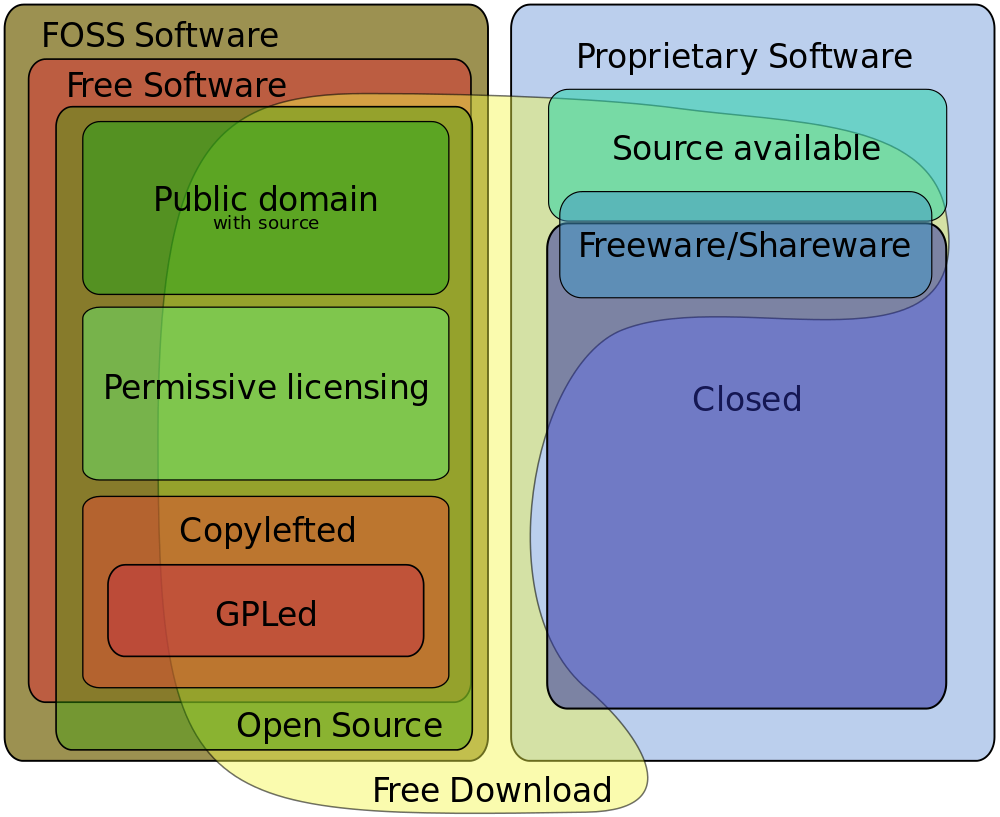
\includegraphics[width=0.5\linewidth]{figs/Software_Categories_expanded}
      \caption{Diagram of software under various licenses according to the FSF and their The Free Software Definition: on the left side "free software", on the right side "proprietary software". On both sides, and therefore mostly orthogonal, "free download" (Freeware). CC0, \href{https://commons.wikimedia.org/w/index.php?curid=46544815}{https://commons.wikimedia.org/w/index.php?curid=46544815}}
      \label{fig:software-licenses}
    \end{figure}
    
    Good discussion of software licenses is available at \href{https://en.wikipedia.org/wiki/Software_license}{this Wikipedia article}.
    
    And good comparison of different open-source software licenses is in \href{https://en.wikipedia.org/wiki/Comparison_of_free_and_open-source_software_licenses}{this Wikipedia article}.
    
    Typically the \href{https://en.wikipedia.org/wiki/Apache_License}{Apache License of the Apache Software Foundation} or \href{https://en.wikipedia.org/wiki/Python_Software_Foundation_License}{Python Software Foundation} license are good choices for a `''permissive'' license.  
    
    But the Gnu General Public License \href{https://en.wikipedia.org/wiki/GNU_General_Public_License}{GPLv2 and GPLv3}  are ``stronger'' free and open source software licenses. This is the original free software license written by \href{https://en.wikipedia.org/wiki/Richard_Stallman}{Richard Stallman}  of the \href{https://en.wikipedia.org/wiki/Free_Software_Foundation}{Free Software Foundation} for the \href{https://en.wikipedia.org/wiki/GNU_Project}{GNU Project}.
    
      \begin{figure}[h]
        \centering
        
\includegraphics[width=0.25\linewidth]{figs/Heckert_GNU_white}
        \caption{GNU mascot, by Aurelio A. Heckert}
        \label{fig:gnu-mascot}
      \end{figure}
    
    
  \pagebreak
    \subsection{Scoring Rubric for Oral Presentation}
    Presenter Name:   \\
    Date: \\
    Evaluator Name: 
    
      \subsubsection{Scientific/Technical Content \emph{(25 points)}, And Data Science Content \emph{(25 points)}}
      
      Introduction: 
        \begin{itemize}   \itemsep0pt
            \item{Defines background and importance of research.}
            \item{States data analytics objective}
            \item{Able to identify relevant questions.}
        \end{itemize}
        
      \noindent Body:
        \begin{itemize}  \itemsep0pt
            \item{Presenter has a data analytic goal (EDA, Modeling, Classification).}
            \item{Addresses audience at an appropriate level (rigorous, but generally understandable to a scientifically-minded group).}
            \item{Offers evidence of methods tried, what worked.}
            \item{Describes methodology and implementation.}
            \item{The talk is logical well organized.}
        \end{itemize}
      
      \noindent Conclusion:
        \begin{itemize}  \itemsep0pt
            \item{Summarizes major points of talk.}
            \item{Summarizes potential weaknesses (if any) in findings.}
            \item{Provides you with a “take-home” message.}
        \end{itemize}
      
      \subsubsection{Coding Elements \& Style, .R, .Rmd \emph{(25 points)}}
        \begin{itemize}  \itemsep0pt
            \item{Code author, license, versioning.}
            \item{Code styling, identing, commenting.}
            \item{Is it reproducible code, and well structured data.}
            \item{Cross-platform, cross-computer code: relative paths, or absolute paths}
            \item{Making and using functions.}
            \item{Use of interesting packages}
        \end{itemize}
      
      \subsubsection{Presentation Quality, Clarity, Style (25 pts)}
        \begin{itemize}  \itemsep0pt
            \item{Graphs/figures are clear and understandable.}
            \item{The text is readable and clear.}
            \item{Audio/Visual components support the main points of the talk.}
            \item{Appropriate referencing of data that is/was not generated by presenter}
        \end{itemize}
      
      \subsubsection{General  Comments}
        \begin{flushright}
         Final Score:  ..............  / 100
        \end{flushright}
        
  

%-----------------------------------------
\pagebreak


\section{Setting up your R data science computer}
  If you do want to install the softwares on your personal computer, here's how.
  \subsection{For Windows}
    In Windows we are allowed to use spaces in filenames, however, most other systems does not support that. 
    To avoid conflicts or troubles, we suggest using \href{https://sanaulla.info/2008/06/25/camelcase-notation-naming-convention-for-programming-languages/}{camelBack} naming convention or use "-" or "\_" to replace spaces. 
    
  \subsubsection{LaTeX}
    \LaTeX~is a document preparation system that is widely used in the academia for producing scientific documents. 
    You will need to install two softwares,  Miktex and TeXstudio. \\
    \begin{itemize}
  	\item Download and run the Basic MiKTeX Installer. 
    MiKTeX has the ability to install missing packages automatically, i.e., this installer is suitable for computers connected to the Internet. 
    Before you run the installer, you can check the \href{https://miktex.org/kb/prerequisites-2-9}{prerequisites}. 
    The installer is available on the \href{https://miktex.org/download}{download} page. 
    You start it with a double-click on the downloaded file. 
  	\item Read the Copying Conditions carefully and click "I accept the MiKTeX copying conditions", the click "Next", as demonstrated below. 
  	
    \begin{figure}[!ht]
    	\centering
    	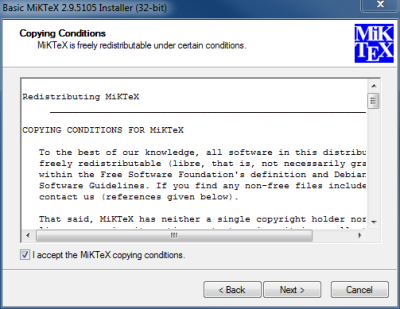
\includegraphics[width=0.7\linewidth]{figs/basic-miktex-license-2-9}
    	\caption{}
    	\label{fig:basic-miktex-license-2-9}
    \end{figure}
    	\item You have the Option to create a shared MiKTeX installation. 
      Click "Anyone who uses this Computer (all users), if you want to install MiKTeX for all users. 
      Click "Only for ...", if you want to install MiKTeX for yourself only. 
      When you have made your decision, click "Next" to go to the next page. 
    	
    \begin{figure}[h]
    	\centering
    	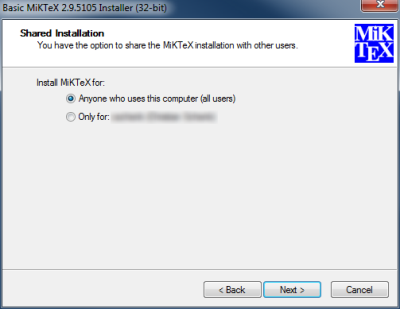
\includegraphics[width=0.7\linewidth]{figs/basic-miktex-shared-2-9}
    	\caption{}
    	\label{fig:basic-miktex-shared-2-9}
    \end{figure}
    
    \pagebreak
    
    	\item You can specify the directory where you want to install your Miktex. 
      Click "Browse", if you want to specify another (than the default) directory location. 
      Click "Next", to go to the next page.
    
    \begin{figure}[!h]
    	\centering
    	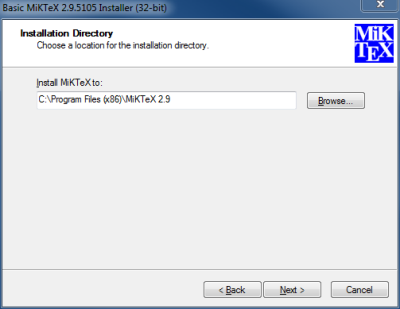
\includegraphics[width=0.7\linewidth]{figs/basic-miktex-installdir-2-9}
    	\caption{}
    	\label{fig:basic-miktex-installdir-2-9}
    \end{figure}
    \pagebreak
    	\item The installer allows you to set the preferred paper size(usually it's A4 in China and letter size in the US). 
      You also have the option to change the default behavior of the integrated package manager for the case where a required package is missing. 
      Select "Yes", to make the package manager is always allowed to install missing packages. 
      All these configurations can be changed later.
    	
    	Click "Next", to go to the next page.
    
    \begin{figure}[h!]
    	\centering
    	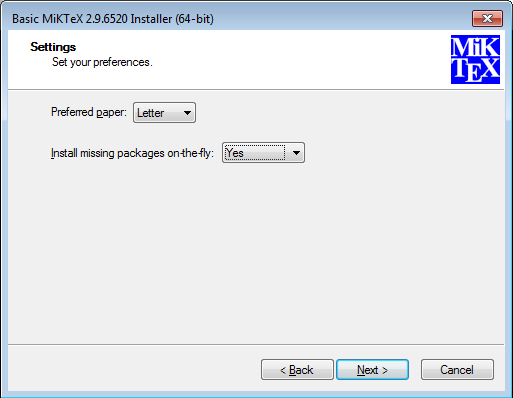
\includegraphics[width=0.7\linewidth]{figs/MikTex1.png}
    	\caption{}
    	\label{fig:basic-miktex-settings-2-9}
    \end{figure}
    	\item Before the actual installation process begins, you get a chance to review your decisions. 
      If you are satisfied with the settings, then click "Start" to start the actual installation. 
    	\item The installation will take a few minutes. 
      The progress bar shows an approximate percentage of completion. 
      When the installation has finished, you can click "Next" to open the last page.
    	\item MiKTeX is now installed. 
      Click "Close", to close the installer.
    	\item In order to make use of latex the easiest way is to use a integrated development editor (IDE). 
      \textbf{TeXstudio} is an free package that allows you to edit tex documents, compile and view them, it has syntax highlighting, auto completion, in line spell and grammar checker and much more. 
      You can find the downloads page \href{https://www.texstudio.org/}{here} and click on \textbf{download now}. 
    	\item Once downloaded, run and start the installer. 
    	\item Accept all the default conditions, and start up TeXstudio to finish. 
    	\item If you need instructions on how to start using LaTeX, here are some \href{https://en.wikibooks.org/wiki/LaTeX}{tutorials}. 
    \end{itemize}
  
  \pagebreak
  \subsubsection{Git}
  
    \textbf{Git Bash} is command line programs which allow you to interface with the underlying git program. 
    Bash is a Linux-based command line, which has been ported over to Windows. 
    \begin{itemize}
    	\item  Download latest version of Git Bash on the \href{http://gitforwindows.org/}{official website}. 
    	\item Once Git Bash Windows installer is downloaded, run the executable file and follow the setups:
    	\item Agree to the GNU General Public License and click "Next". 
    		\begin{figure}[h!]
    			\centering
    			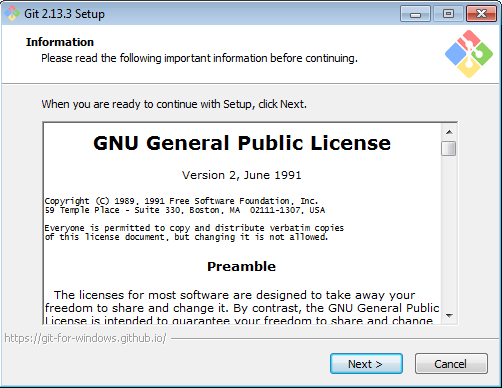
\includegraphics[width=0.58\linewidth]{figs/GitBash1}
    			\caption{}
    			\label{fig:gitbash1}
    		\end{figure}
    	\item Select the location where you want to install the Git Bash. 
    		\begin{figure}[!h]
    			\centering
    			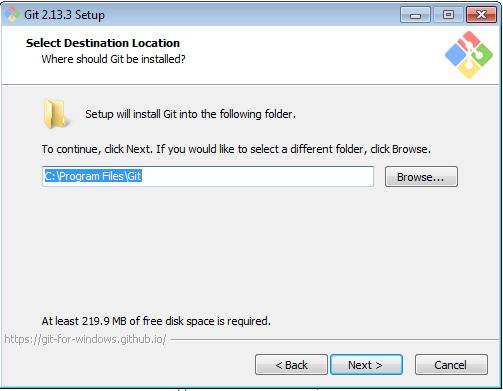
\includegraphics[width=0.58\linewidth]{figs/GitBash2}
    			\caption{}
    			\label{fig:gitbash2}
    		\end{figure}
    	
    	\pagebreak
    	\item Select the components you want to install and click Next. 
      We suggest that you should unselect Windows Explorer integration. 
    		\begin{figure}[h!]
    			\centering
    			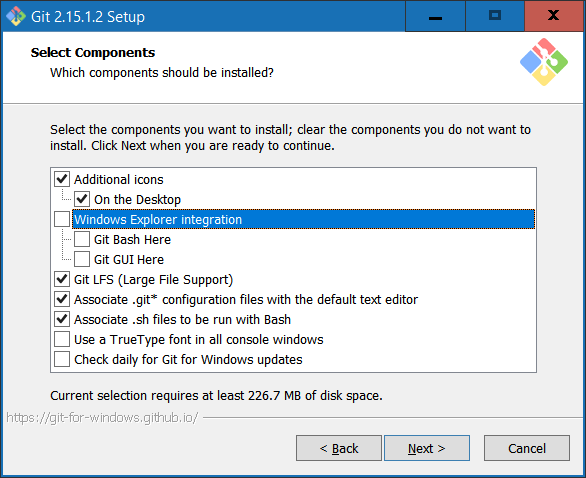
\includegraphics[width=0.65\linewidth]{figs/git2}
    			\caption{}
    			\label{fig:gitbash3}
    		\end{figure}
    	\item Set default editor to Vim(which is the default option). 
    		\begin{figure}[h!]
    			\centering
    			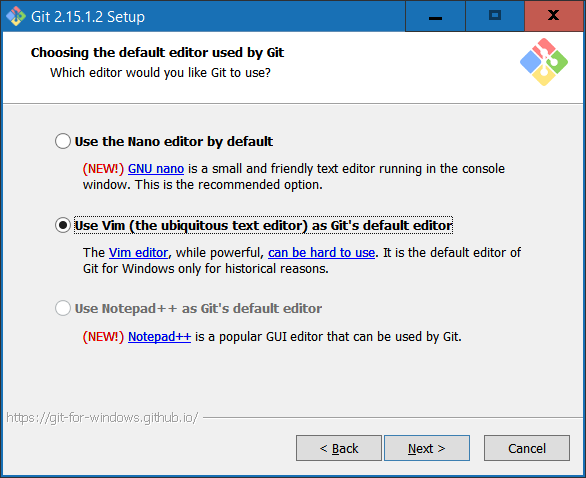
\includegraphics[width=0.65\linewidth]{figs/git1}
    			\caption{}
    			\label{fig:gitbash4}
    		\end{figure}
    
    	\pagebreak
    	\item We suggest that you use the default option, which is "Use Git from Git Bash only". 
    		\begin{figure}[h!]
    			\centering
    			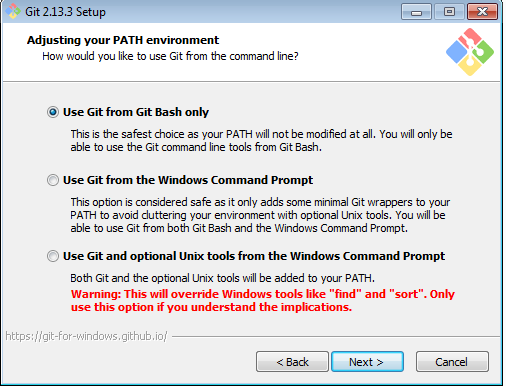
\includegraphics[width=0.7\linewidth]{figs/GitBash5}
    			\caption{}
    			\label{fig:gitbash5}
    		\end{figure}
    	\item Select which SSL/TLS library would you like to use for HTTPS connection and click Next. 
    	
    		\begin{figure}[h!]
    			\centering
    			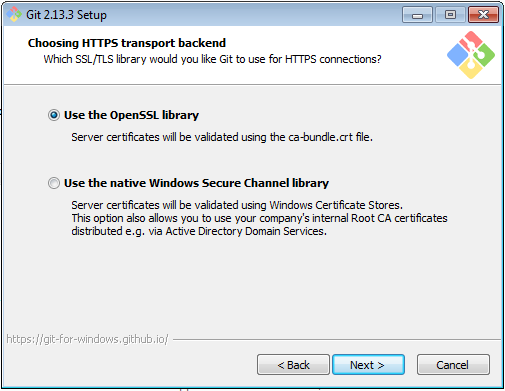
\includegraphics[width=0.7\linewidth]{figs/GitBash6}
    			\caption{}
    			\label{fig:gitbash6}
    		\end{figure}
    
    	\pagebreak
    	\item Select, how should Git treat line endings in text files and click Next. 
    		\begin{figure}[h!]
    			\centering
    			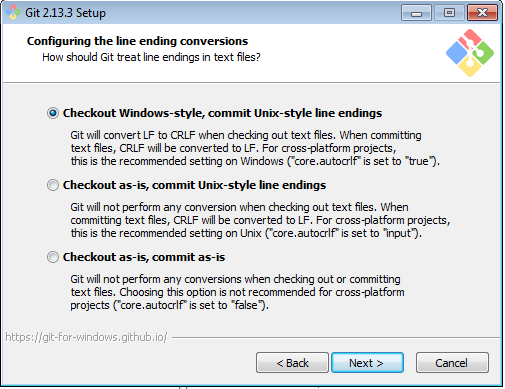
\includegraphics[width=0.7\linewidth]{figs/GitBash7}
    			\caption{}
    			\label{fig:gitbash7}
    		\end{figure}
    	\item Select the terminal you want to use for Git Bash. 
    
    		\begin{figure}[h!]
    			\centering
    			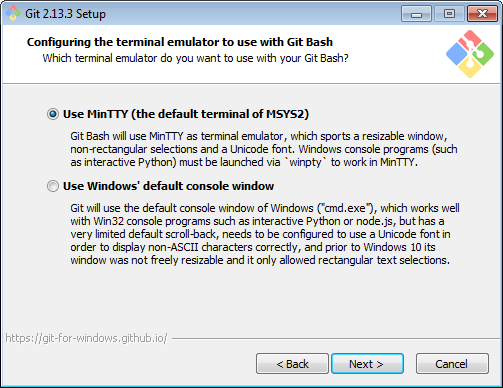
\includegraphics[width=0.7\linewidth]{figs/GitBash8}
    			\caption{}
    			\label{fig:gitbash8}
    		\end{figure}
    	\pagebreak
    	\item Select the features you want to enable and click "Next". 
      We suggest that you unselect "Enable Git Credential Manager". 
    		\begin{figure}[h!]
    			\centering
    			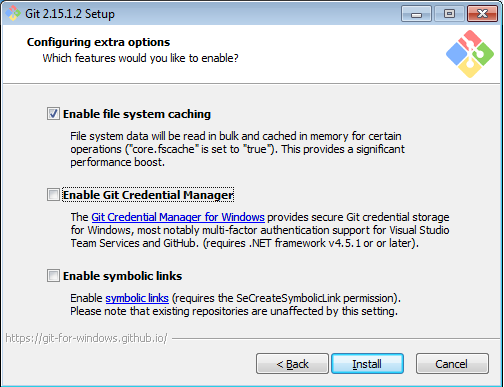
\includegraphics[width=0.7\linewidth]{figs/git4}
    			\caption{}
    			\label{fig:gitbash9}
    		\end{figure}
    
    	\item Please wait while Setup wizard installs Git on your computer and click "Finish" to exit the Setup wizard. 
    	\item After Git Bash installation finishes you will ready to use the Linux command on a windows machine. 
      Double click on below icon to start the Git Bash. 
    		\begin{figure}[h!]
    			\centering
    			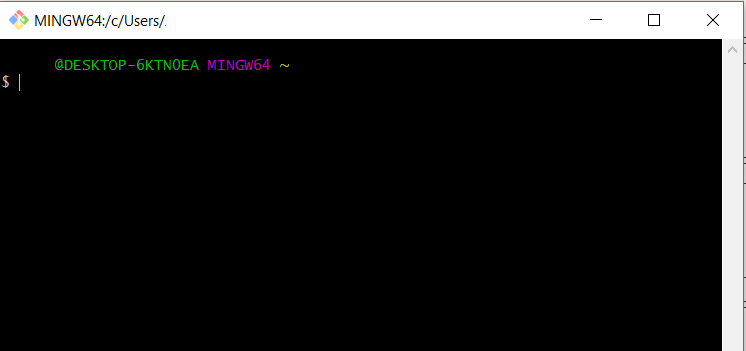
\includegraphics[width=0.7\linewidth]{figs/Launch-Git-Bash.png}
    			\caption{}
    			\label{fig:launchgitbash}
    		\end{figure}
    	\item Set up user name and email in Git.
    	\begin{lstlisting}
    	git config --global user.name "yourusername"
    	git config --global user.email "youremail@website.com"
    	git config --global color.ui auto
    	\end{lstlisting}
    	\item Here are some common commands you can use in git:\\
    		pwd -- present working directory\\
    		cd -- change directory\\
    		ls -- list files in current working directory\\
    		mkdir -- make new directory\\
    	\item If you want to learn more about how git works (pull request, merge and more), you can read some \href{https://www.atlassian.com/git}{tutorials}. 
    	
    \end{itemize}
  
  \subsubsection{R}
    R is a free programming language and software environment for statistical computing and graphics that is supported by the R Foundation for Statistical Computing, while RStudio is a free and open-source integrated development environment for R. 
    \begin{itemize}
    	\item To \href{https://cran.r-project.org/}{download R}, please choose your "install R for Windows" and then choose base R for a complete installation. 
    	\item Double click on the installer, and follow the instructions. 
    	\item Users of Vista/Windows 7/8/Server 2008/2012 installing for a single user using an account with administrator rights should consider installing into a non-system area (such as C:\textbackslash R). 
    	\item Please try to avoid spaces or any special characters other than English letters and numbers in your installation directory, which may cause error later.
    	\item After installing R, you can download \textbf{Rstudio} \href{https://www.rstudio.com/products/rstudio/download/}{here}, and choose the RStudio Desktop Open Source License version (the left most one). 
    	\item Run the installer and follow the installation instructions.  
    	\item Again, please try to avoid spaces or any special characters other than English letters and numbers in your installation directory. 
    	\item Rstudio have some built-in packages such as tidyverse and ggplot2, but if you are interested in building your own R packages, you can \href{https://cran.r-project.org/bin/windows/Rtools/}{download \textbf{Rtools}}. Please choose the latest version, as the older versions are not compatible with latest release of R. 
    	\item Run the installer, and accept the defaults throughout. 
    	\item Confirm and finish the installation. 
    	\item Once the Rtools installation completes, open RStudio and go to Profile--Global options--Code and change the code editing options as follows:
    	
    	\begin{figure}[h!]
    		\centering
    		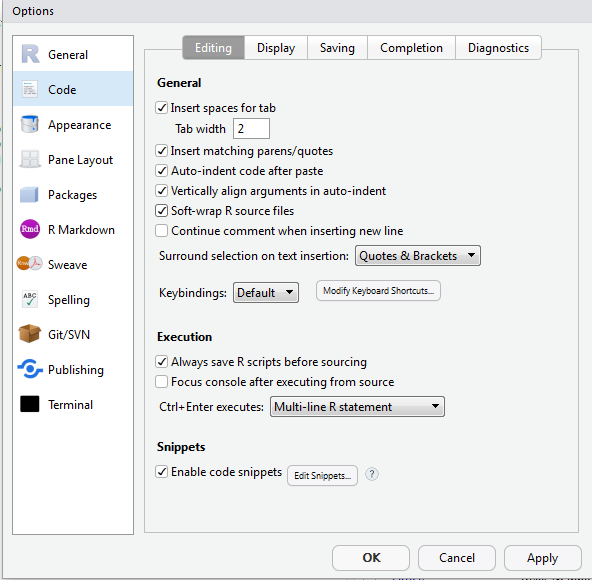
\includegraphics[width=0.6\linewidth]{figs/softwrapRsourcefile}
    		\caption{}
    		\label{fig:softwraprsourcefile}
    	\end{figure}
    	\pagebreak
    %	\item To install devtools, use 
    %	\begin{lstlisting} 
    %	install.packages("devtools")
    %	\end{lstlisting}
    	\begin{figure}[h!]
    		\centering
    		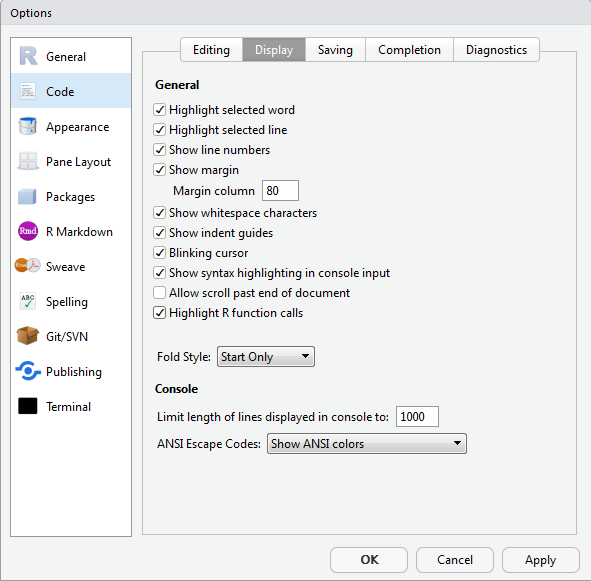
\includegraphics[width=0.6\linewidth]{figs/highlightRfunctioncall}
    		\caption{}
    		\label{fig:highlightrfunctioncall}
    	\end{figure}
    	\pagebreak
    	\item You can also change your appearance style in Global Options:
    	
    	\begin{figure}[h!]
    		\centering
    		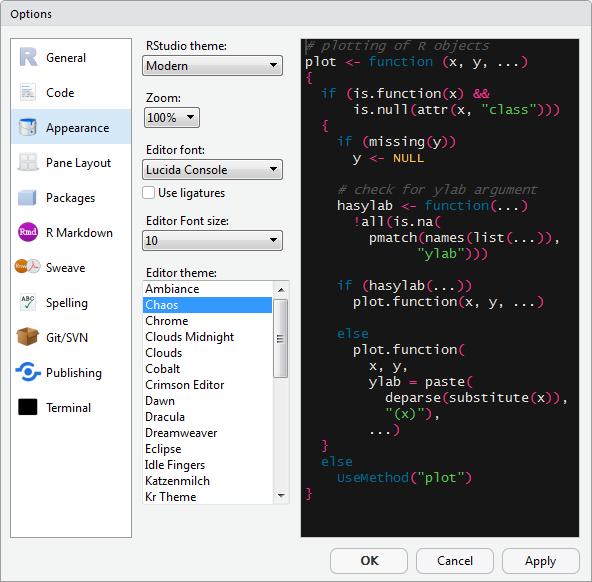
\includegraphics[width=0.6\linewidth]{figs/chaos}
    		\caption{}
    		\label{fig:chaos}
    	\end{figure}
    	\item Here is the list of standard packages that we suggest you install. 
      If a warning comes up asking whether you want to install packages from the source, answer "y" for yes. \\
      
    	Alphabetical packages:\\
      
        acepack 
        adabag
        akima
        AmesHousing
        animation
        anytime
        arules
        aspace
        astsa
        available
        bagRboostR
        baseline  
        BayesFactor
        bayesSurv
        BayHaz 
        bcpa
        bda 
        birk
        bit64
        blogdown
        BMA
        bookdown
        bookdownplus
        BoomSpikeSlab
        boot
        bootstrap
        breakDown
        breakpoint
        brms  
        broom
        bsts
        C50
        Cairo
        car
        caret 
        caretEnsemble
        CausalImpact
        centiserve
        changepoint
        changepoint.np
        ChemoSpec
        cgwtools
        class
        ClimClass
        cloudml
        cluster.datasets 
        coda
        CORElearn 
        corrgram 
        corrplot
        cowplot
        cpca
        ctv
        CVXR
        data.table
        data.tree 
        dataMaid
        DBI
        DBItest
        dbscan
        ddiv
        devtools 
        DiagrammeR
        DiagrammeRsvg
        dice
        digest 
        DMwR
        doParallel
        dplyr 
        DT
        dummies
        dtwclust
        e1071
        eemR 
        ElemStatLearn
        epiDisplay
        factoextra
        fastcluster 
        feather
        flexclust 
        forecast
        foreach
        gam
        gapminder
        gbm 
        gclus 
        GGally 
        gganimate
        ggbiplot   
        ggforce
        ggmap 
        ggplot2
        ggpubr
        ggQC
        ggRandomForest
        ggraph
        ggridges
        ggthemes
        ggvis 
        glmnet 
        gmodels 
        googleVis  
        graphlayouts
        gridBase 
        gridExtra 
        gsl
        gstat
        gWidgets
        h2o
        HadoopStreaming  
        HarmonicRegression
        hcp 
        hdpca
        hexbin  
        HH 
        httr 
        htmlwidgets
        htmltools
        hyperSpec 
        igraph
        infer 
        ipred 
        IQCC 
        IRkernel
        ISLR 
        itertools 
        jsonlite
        kableExtra
        keras
        kerasformula
        kerasR
        kernlab 
        keyring
        kgc
        klaR 
        knitcitations 
        knitr 
        Lahman
        lars 
        lavaan 
        lavaan.survey 
        leaps
        learningr
        learNN
        learnBayes
        lime 
        lintr 
        lme4 
        lobstr
        logitnorm 
        magick
        magrittr 
        Make 
        mapdata
        Mapmate
        mapproj
        maps
        markdown
        maptools
        MASS 
        Matrix 
        MatrixModels 
        matrixStats 
        markovchain
        mcmc
        MCMCglmm
        metRology
        Metrics
        mgcv
        minpack.lm
        MTS
        multiway
        NbClust
        netSEM
        neural 
        neuralnet 
        NeuralNetTools
        nnet
        nycflights13
        odbc
        OIdata  
        olsrr
        OIsurv 
        onehot
        OneR
        onlineCPD
        openintro 
        optimx
        optiRum
        packHV
        packrat 
        pacman
        parallelSVM
        patchwork
        pca3d    
        PerformanceAnalytics
        pipeR 
        plot3D 
        plotmo
        plotKML
        plotly
        pls
        Plumber
        plyr
        plyrmr
        png
        pool
        prodlim
        pROC
        prophet
        profvis
        propagate
        proxy
        pryr
        psych  
        purrr
        qcc 
        qtlmt
        qualityTools   
        quantmod 
        r2d3
        randomForest
        randomForestSRC
        ranger
        raster
        rasterVis
        rCharts
        RColorBrewer 
        Rcpp 
        RCurl
        Rdice
        Rdpack
        readr
        recipes
        RefManageR
        relaimpo
        reshape 
        reshape2 
        reticulate
        rgdal
        rgexf
        rgeos 
        rggobi 
        rgl 
        rJava 
        rjson
        RJSONIO 
        jsonvalidate
        rlist 
        RLRsim
        rmarkdown 
        Rmisc
        Rmpi
        rms
        RMySQL 
        RNiftyReg   
        rNMF 
        roxygen2 
        rpart 
        rprojroot
        rPython 
        rsample
        RSNNS
        rstan
        rstanarm
        rsvg
        RTest
        RTextTools
        rticles
        Rtsne
        rtweet
        RUnit
        rvest   
        rworldmap
        rworldxtra
        scatterplot3d  
        scrypt 
        segmented 
        sem 
        shiny
        shinydashboard
        shinyjs
        shinystan
        shinytest
        shinythemes
        signal
        simpleNeural
        SixSigma  
        sp 
        sparklyr
        sparktf
        spc 
        spelling
        sqldf  
        sqliter
        sqlutils 
        stationaRy 
        statsr
        stlplus
        stockPortfolio 
        StreamMetabolism
        stringi
        stringr
        styler
        survival
        survivAll 
        survivalAnalysis 
        survivalMPL 
        survivalROC 
        survivalsvm
        survminer 
        svglite
        svUnit
        SwarmSVM
        synthpop
        TeachingDemos
        TeachingSampling
        tensorflow
        testthat
        tfdatasets
        tfdeploy
        tfestimators
        tfruns 
        tibble
        tictoc
        tidyGraph
        tidymodels
        tidyposterior
        tidyr 
        tidytext
        tidyverse
        tidygraph
        timeDate
        timevs
        tinytex
        tm
        transformr
        tree 
        TSclust
        TSstudio
        tweenr
        tweezer
        validate
        vtreat
        WaveletComp
        wavelets
        wavethresh
        wmtsa
        WGCNA
        WDI 
        wordcloud 
        XLConnect  
        XML 
        xtable
        xts 
        yardstick
        zipcode
        zoo 
  
  	You can go to the highlighted tab in the below picture and install-upgrade your packages here. 
    
    To install, simply paste the list of packages in the window. 
  
  	\begin{figure}[h!]
  		\centering
  		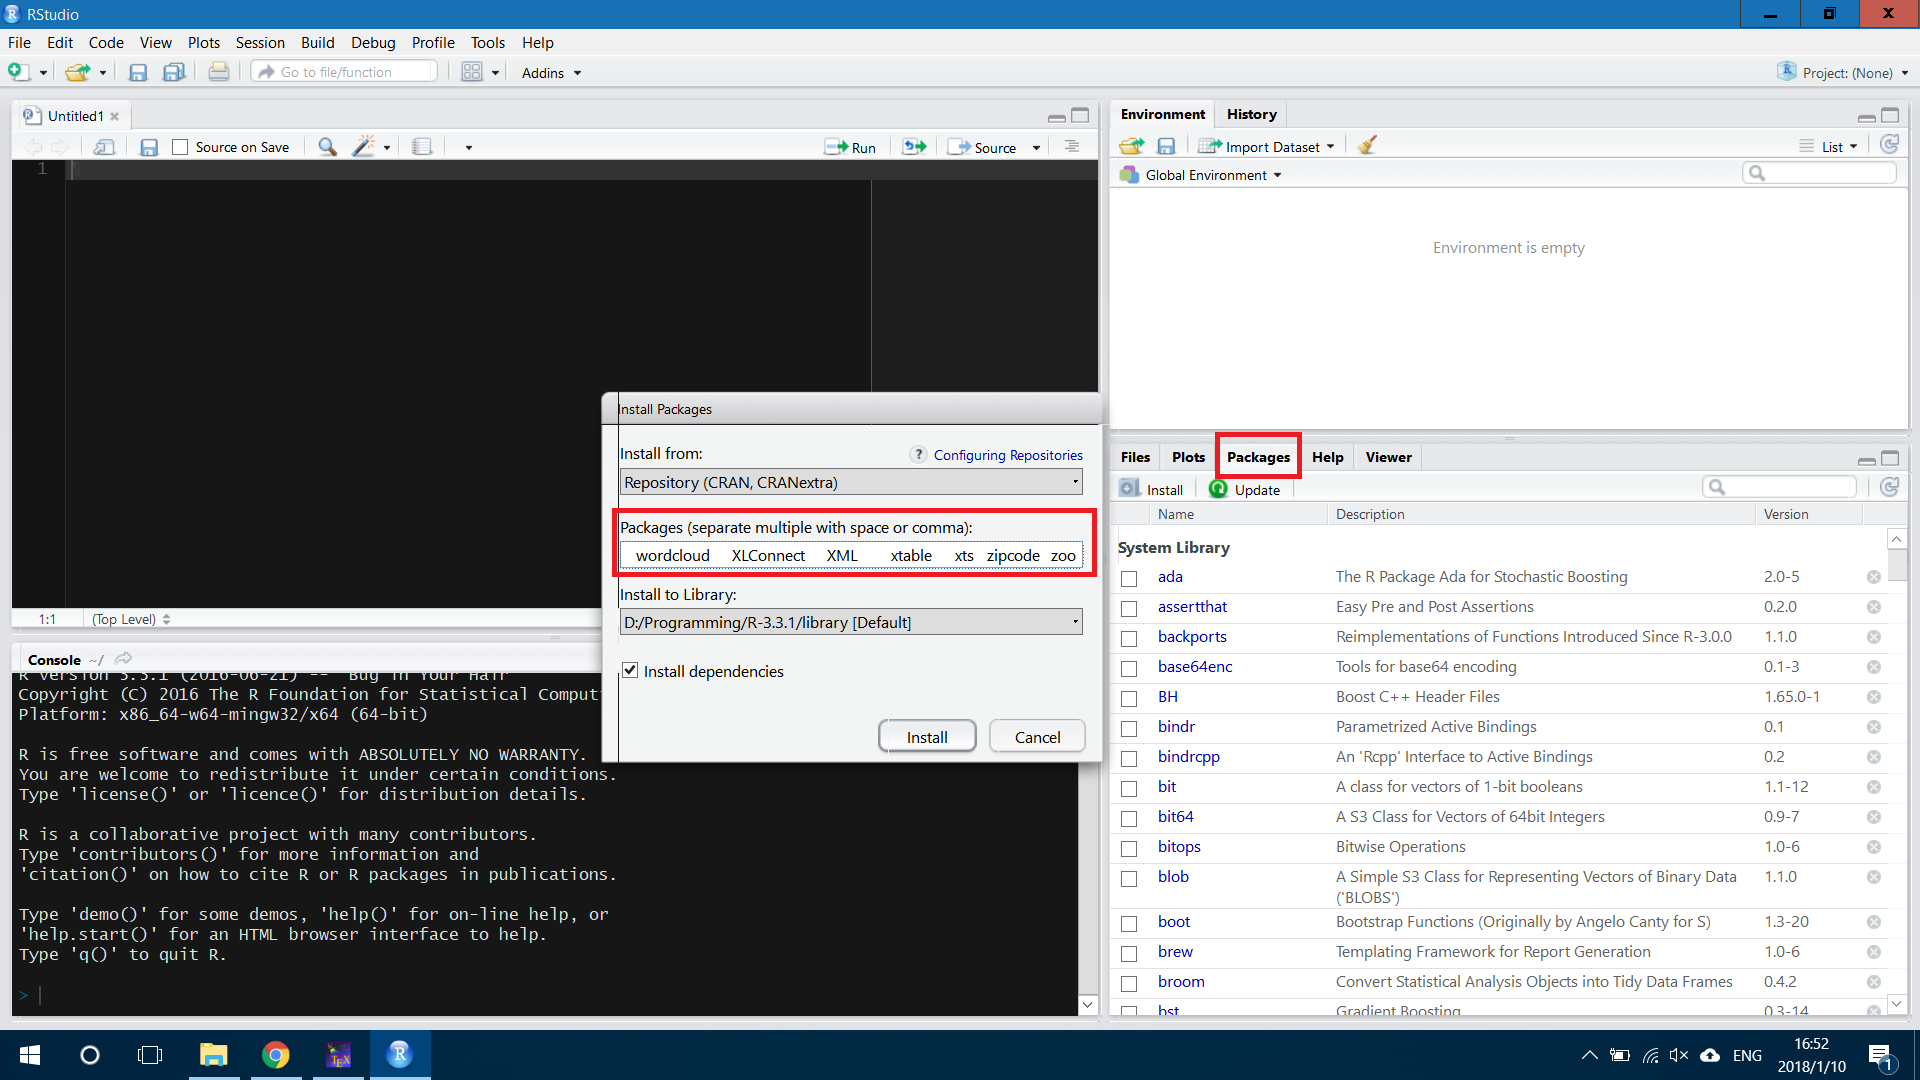
\includegraphics[width=0.7\linewidth]{figs/installPackages}
  		\caption{}
  		\label{fig:installpackages}
  	\end{figure}
  	
  	To upgrade your packages, select all packages and press "Install Updates"
  		
  	\begin{figure}[h!]
  		\centering
  		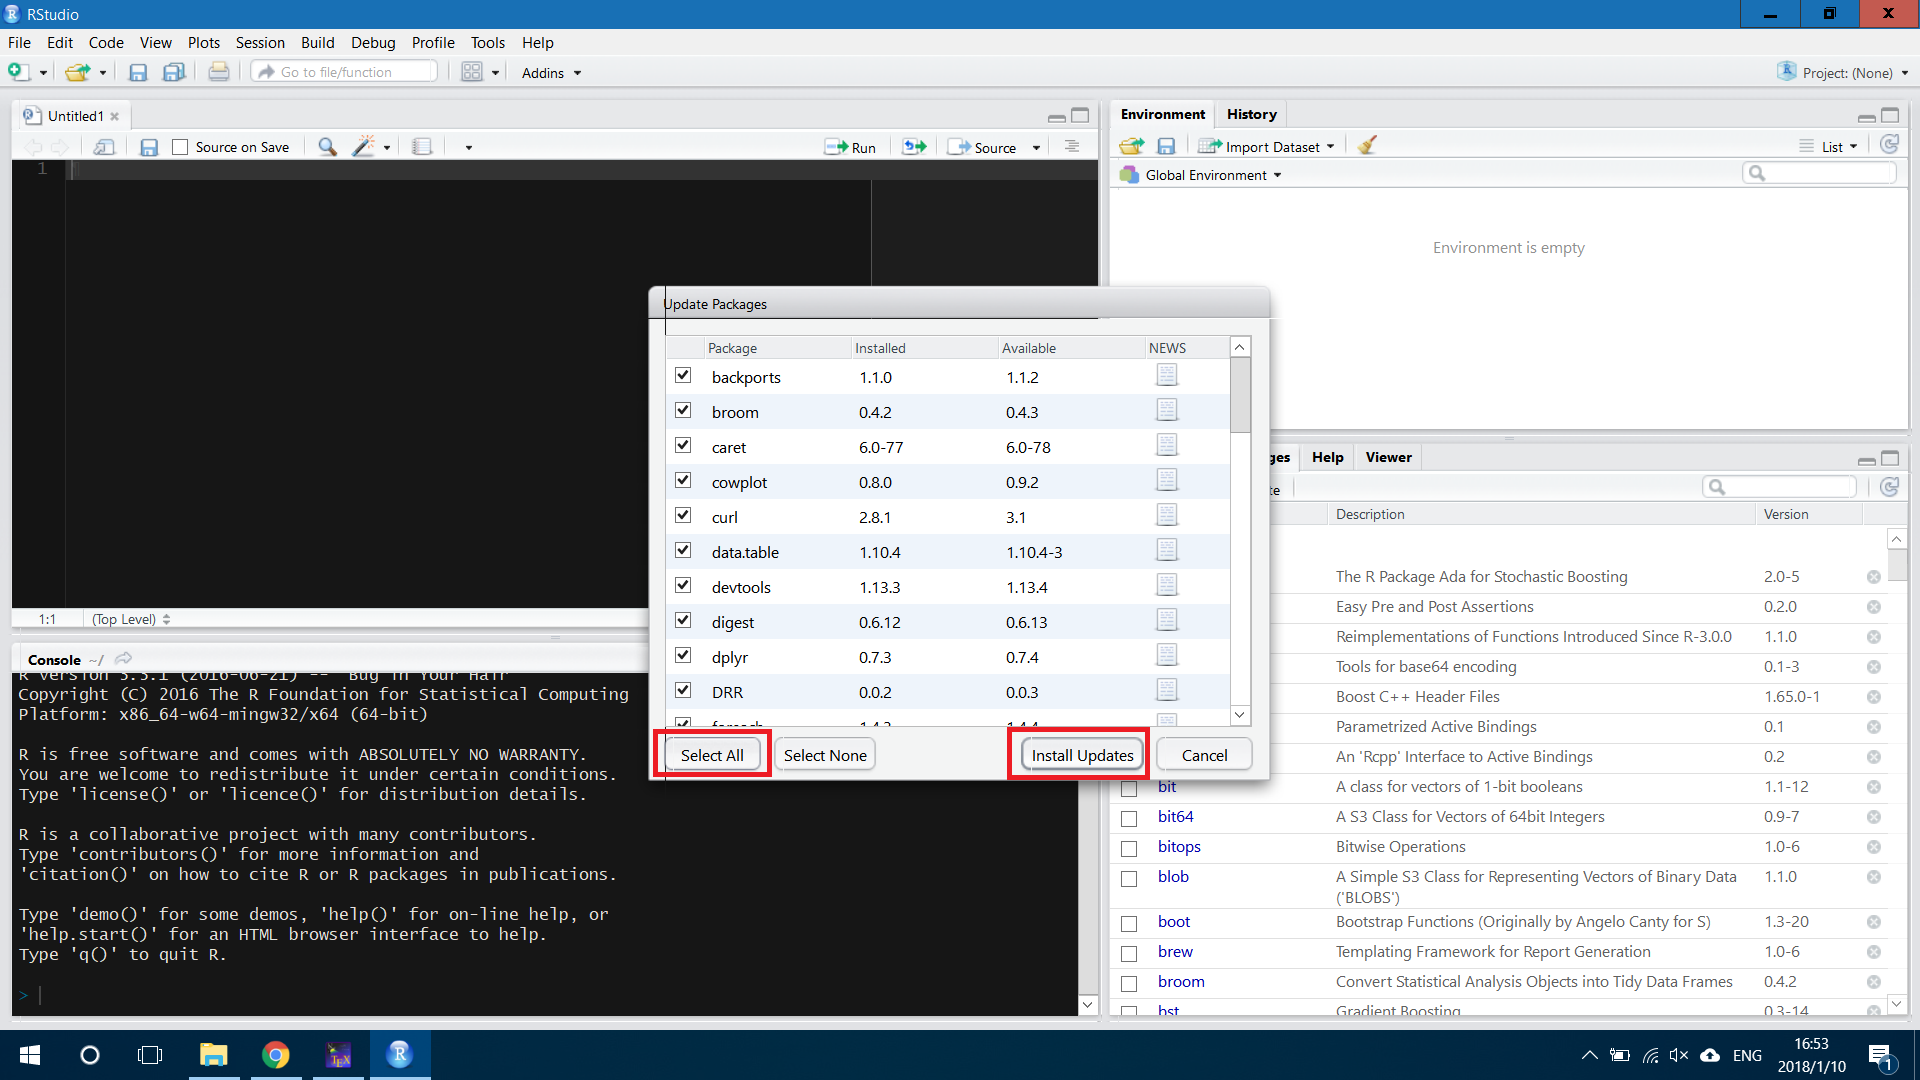
\includegraphics[width=0.7\linewidth]{figs/upgradePackages}
  		\caption{}
  		\label{fig:upgradepackages}
  	\end{figure}
  
%    \item A few packages from git hub
%    
%    Install gganimate: devtools::install\_github("dgrtwo/gganimate")
%  
%    Install MLstudio: devtools::install\_github("RamiKrispin/MLstudio")
%  
%    Install TSstudio: devtools::install\_github("RamiKrispin/TSstudio")
  
  
    \end{itemize}
  
    \subsubsection{GVim}
    GVim offers a graphic user interface for the editor \textbf{Vim}. 
    This is a powerful editor but could be a little bit hard to use. 
    \begin{itemize}
    	\item You can download Vim from their \href{https://vim.sourceforge.io/download.php}{download page}. 
      For Windows system, click on "\href{https://vim.sourceforge.io/download.php#pc}{PC: MS-DOS and MS-Windows}", and download "gvim80.exe". 
    	\item Open the installer and accept the default conditions. 
    \end{itemize}
    
  \subsection{For Linux}
  
    \subsubsection{LaTeX}
    TeX Live is an easy way to get up and running with the TeX document production system, it is available on most Unix-like systems, but it is recommended to use MacTeX if you are using MacOSX. 
    To install TeXLive and TeXstudio, run the following code:
    	\begin{lstlisting}
    	sudo apt-get install texlive-full texworks texstudio
    	\end{lstlisting}
      
  \subsubsection{Git}
    To install Git, run the following code:
    	\begin{lstlisting}
    	 sudo apt-get install git
    	\end{lstlisting}
      
  \subsubsection{R}
  
    \begin{itemize}
    	\item Install from CRAN:
    	\begin{lstlisting}
    	## This sets up the CRAN repository in your Linux Package Manager
    	sudo echo "deb http://cran.rstudio.com/bin/linux/ubuntu xenial/" | 
    	sudo tee -a /etc/apt/sources.list
    	gpg --keyserver keyserver.ubuntu.com --recv-key E084DAB9
    	gpg -a --export E084DAB9 | sudo apt-key add -
    	sudo apt-get update
    	sudo apt-get install r-base r-base-dev
    	## extra linux packages needed by
    	sudo apt-get install r-cran-xml  pkg-config libxml2-dev
    	libtiff5-dev fftw3 fftw3-dev  tmux libav-tools
    	cifs-utils openssh-server openssh-client tree htop
    	gdebi curl libcurl4-openssl-dev libssl-dev
    	\end{lstlisting}
    	\item Before installing, you should \href{https://www.rstudio.com/products/rstudio/download/}{check the latest version} of RStudio, and change the version number in the code below accordingly. 
      Install RStudio:
    	\begin{lstlisting} 
    	## Update to the latest version number in the lines below
    	wget https://download1.rstudio.org/rstudio-1.1.383-amd64.deb
    	sudo gdebi -n rstudio-1.1.383-amd64.deb
    	rm rstudio-1.1.383-amd64.deb
    	\end{lstlisting}
    
    \end{itemize}
  
  \subsection{For Mac}
  
    \subsubsection{Homebrew}
      Homebrew is a package manager for Mac OS. 
      To install Homebrew, paste and run the following command in terminal:
      \begin{lstlisting}
      /usr/bin/ruby -e "$(curl -fsSL https://raw.githubusercontent.com/Homebrew/
      install/master/install)"
      \end{lstlisting}
      You can read more about Homebrew \href{https://brew.sh/}{here}.
    
    \subsubsection{XQuartz}
      To correctly set up your linux environment, you should also install XQuartz.
      XQuartz is Apple Inc.'s version of the X server, a component of the X Window System for macOS. 
      You can \href{https://www.xquartz.org/}{download} and install the latest version of XQuartz. 
    
    \subsubsection{LaTeX}
      To install LaTeX on Mac, you need to install MacTeX and TeXstudio. 
      \begin{itemize}
      	\item The current distribution as of today (\today)is MacTeX-2017. 
        This distribution requires Mac OS 10.10, Yosemite, or higher and runs on Intel processors. 
        To download, click \href{http://www.tug.org/mactex/mactex-download.html}{MacTeX Download}. 
      	\item After downloading, double click on the MacTeX.pkg to install. 
        Follow the straightforward instructions. 
        Installation on a recent Macintosh takes four to six minutes. 
      	\item At the end of installation, the installer will report "Success." But sometimes, the installer puts up a dialog saying "Verifying..." and then the install hangs. 
        In all cases known to us, rebooting the Macintosh fixes this problem. 
        After the reboot, install again. 
      	\item Now you can start installing TeXstudio. 
        You can find the corresponding installer on the \href{https://www.texstudio.org/}{TeXstudio website}. 
      	\item Because the developers of TeXstudio do not have an Apple Developer Account, OS X may complain about an unidentified developer and deny opening TXS. 
        In that case, open the context menu on the TXS icon (Ctrl + Click) and select open. 
      \end{itemize} 
    
    \subsubsection{Git}
      There are several ways to install Git on a Mac. 
      In fact, if you've installed XCode (or it's Command Line Tools), Git may already be installed. 
      To find out, open a terminal and enter git --version. 
      
      Apple actually maintain and ship their own fork of Git, but it tends to lag behind mainstream Git by several major versions. 
      You may want to install a newer version of Git using the method below:
      \begin{itemize}
      	\item Download the latest Git for \href{https://git-scm.com/download/mac}{Mac installer}. 
      	\item Follow the prompts to install Git. 
      	\item Open a terminal and verify the installation was successful by typing git --version. 
      	\item Configure your Git username and email using the following commands, replacing "yourusername" with your own. 
        These details will be associated with any commits that you create:
      	\begin{lstlisting}
      	$ git config --global user.name "yourusername"
      	$ git config --global user.email "youremail@website.com"
      	\end{lstlisting}
      \end{itemize}
    
    \subsubsection{R}
    
      \begin{itemize}
      	\item Download R from \href{http://cran.us.r-project.org/}{CRAN} and click "Download R for (Mac) OS X". 
      	\item Follow the instructions and install R. 
      	\item Download the latest RStudio from their \href{https://www.rstudio.com/products/rstudio/download/}{website}. 
        Open the installer and follow the instructions. 
      \end{itemize}



%-----------------------------------------


\bibliographystyle{ieeetr}
\bibliography{dsci}
%\bibliography{IEEEabrv, EMSE343-443}

\end{document}
